


{\large Slide 06. DIFUSÃO}


\section{Difusão em Sólidos}

\textit{Def:} O transporte de massa no sólido se dá através de movimento atômico.

Casos práticos:

\begin{itemize}
	\item Filtros para purificação de gases;
	\item Modificação superficial de peças;
	\item Dopagem de semicondutores;
	\item Revestimentos.
\end{itemize}



\subsection{Cementação}

\begin{itemize}
	\item Mdificação superficial de peças;
	\item Aumento do teor de C na parte mais externa de engrenagens para aumentar a dureza. Fonte de carbono: pó de grafite ou em fase liquida ou gasosa.
\end{itemize}


\subsection{Galvanização}


Imersão de pelas de aço em zinco fundido formando camadas de ligas Fe-Zn unidas metalurgicamente ao metal base. Temp. 445 a 455 $\degres$ C.

\subsection{Difusão L-L}
O potencia de difusão é dados pelo gradiente de concentração no sistema.


\subsection{Difusão S-S}

Objetivo: Equalização da composição química em ligas. PROCESSO TERMICAMENTE ATIVADO.

\subsubsection{Par de Difusão}

Duas barras de materiais metálicos  distintos sob o tratamento térmico. Concentrações de cobre e de níquel em função da posição no par de difusão. 

\textit{concentrações de cobre e de níquel em função da posição no par de difusão.}


\subsubsection{Condição para ocorrer difusão de átomos na rede cristalina}

\begin{itemize}
	\item Deve haver espaço livre (lacuna) adjacente ao átomo.
	\item O átomo que se desloca deve possuir energia suficiente para quebrar as ligações química que o une a seus átomos vizinhos .
	\item A movimentação dos átomos pode se dar pelo volume do material ou ao longo de defeitos cristalinos (mais rápida).
\end{itemize}


Mecanismos propostos:

\begin{enumerate}
	\item Difusão por lacunas (ou difusão substitucional)
	\item Difusão intersticial
	
\end{enumerate}


\begin{itemize}
	\item Difusão por lacunas (ou difusão substitucional): Átomo se desloca da posição padrão da rede cristalina para algum local (sitio) vazio próximo.
	\begin{itemize}
		\item O átomo segue direção contrária ao movimento da lacuna.
		\item Depende da quantidade de lacunas presentes na rede cristalina.
		\item A quantidade de lacunas aumenta com a temperatura.
		\item O processo é denominado AUTODIFUSÃO quando os próprios átomos da rede se difundem ou INTERDIFUSÃO quando ocorre difusão de impurezas substitucionais.
	\end{itemize}
	\item Difusão intersticial
	\begin{itemize}
		\item Átomos intersticiais migram para posições adjacentes da rede cristalina.
		\item Corresponde a um tipo importante de difusão em metais e ligas cuja impureza apresenta pequeno raio atômico em relação ao átomo da matriz cristalina. (ex: C e H)
		\item É geralmente mais rápida (apresenta maior coeficiente de difusão)
		\item Menor energia necessária para o movimento dos átomos.
	\end{itemize}
\end{itemize}

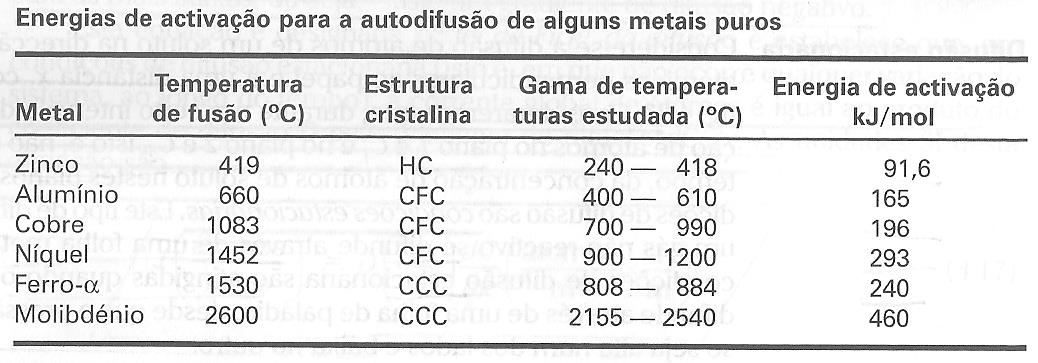
\includegraphics[scale=0.2,trim={0 0 0 0}]{figures/Eativacao}

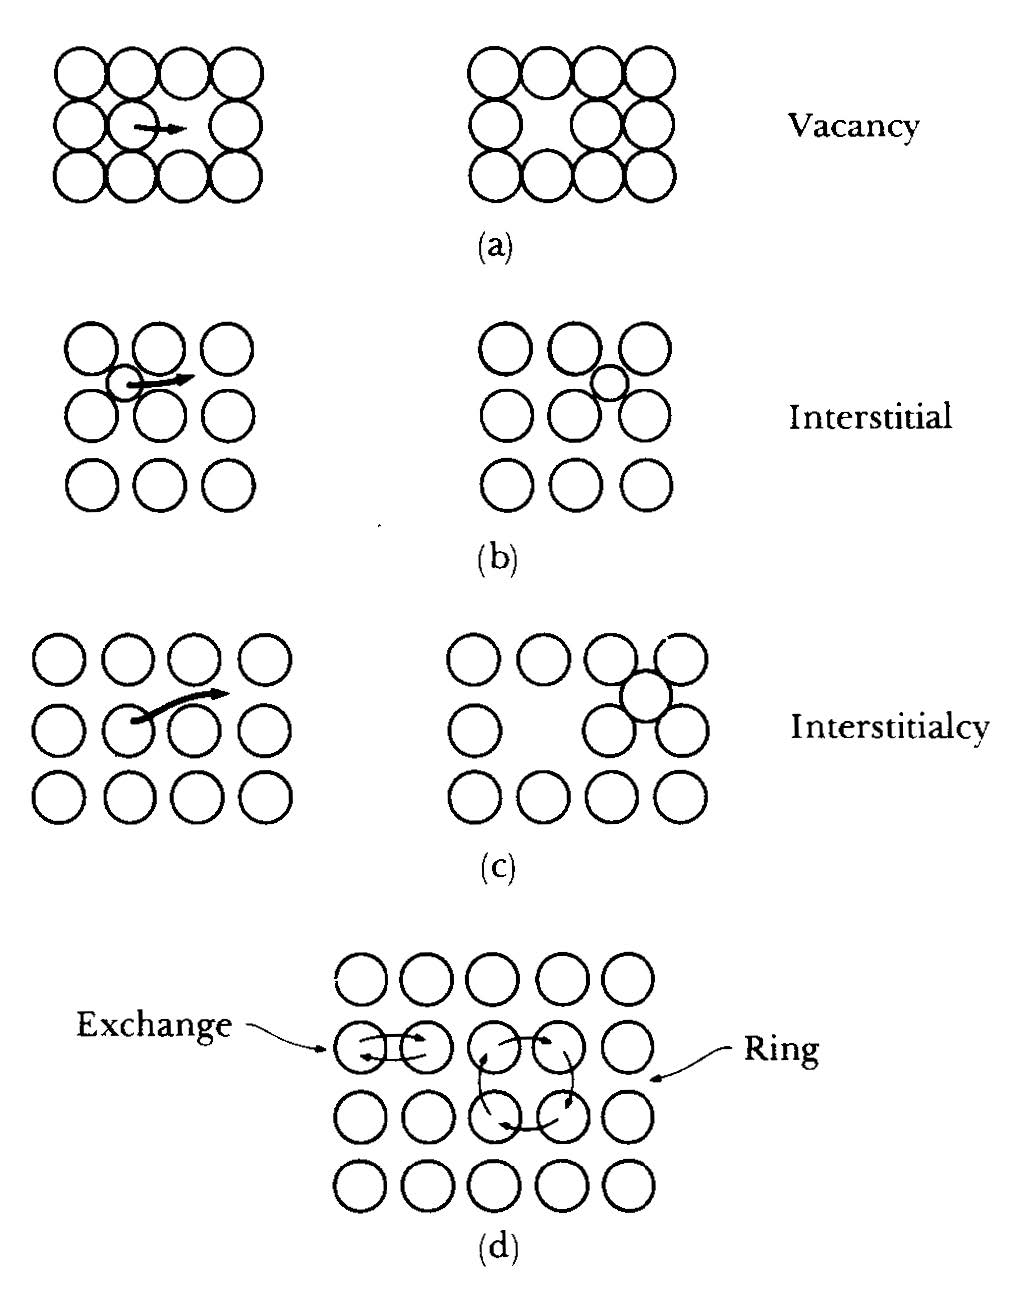
\includegraphics[scale=0.45,trim={0 0 0 0}]{figures/difusao}


\subsubsection{Fluxo de Difusão}

A velocidade com que ocorre a difusão é avaliada em termos de FLUXO DE DIFUSÃO que corresponde a massa (ou número de átomos) que se difunde por unidade de tempo através de uma área perpendicular à direção do movimento da massa que está se difundindo.

\begin{equation}\label{key}
J = \frac{M}{(A \cdot t)}
\end{equation}

onde: 

\begin{itemize}
	\item J = fluxo de difusão. $[\frac{Kg}{m^{2} \cdot s}]$ ou $[\frac{át}{m^{2} \cdot s}]$
	\item M = massa transportada (ou quantidade de átomos)
	\item A = área da seção transversal
	\item t = tempo
\end{itemize}


A velocidade de difusão pode ainda ser avaliada sob duas condições conhecidas na engenharia química:

\begin{itemize}
\item Difusão em estado estacionário
\item Difusão em estado não estacionário (condições transientes)
\end{itemize}

DIFUSÃO EM ESTADO ESTACIONÁRIO

Condições:

\begin{itemize}
	\item J não varia com o tempo.
	\item J não varia com a posição.
\end{itemize}

PRIMEIRA LEI DE FICK: relaciona o fluxo com o gradiente de concentração

\begin{equation}\label{key}
J = D \cdot \frac{\Delta c}{\Delta x}
\end{equation}

onde: 

\begin{itemize}
	\item J = fluxo ($[\frac{atm}{cm^{2}\cdot s}]$)
	\item D = Coeficiente de difusão $[\frac{cm^{2}}{s}]$ - valores tabelados; dependente da temperatura.
	\item $\frac{\Delta c}{\Delta x}$ gradiente de concentração $[\frac{atm}{cm^{3} \cdot cm}]$
	\item O sinal negativo indica que o fluxo ocorre no sentido da maior para a menor concentração.
\end{itemize}

DIFUSÃO EM ESTADO NÃO- ESTACIONÁRIO

Segunda lei de Fick:

\begin{equation}\label{key}
\frac{\partial C}{\partial t}=D \frac{\partial^{2} C}{\partial x^{2}}
\end{equation}



\begin{itemize}
	\item Ocorre na maioria das situações praticas que envolve difusão em sólidos.
	\item Tanto o fluxo de difusão quanto o gradiente de concentração variam com o tempo em uma determinada posição.
	\item Ocorre acúmulo ou esgotamento dos componentes que estão se difundindo.
	\item Sendo especificadas as condições de contorno para a segunda Lei de Fick, podem-se obter soluções que são funções que representam as concentrações em termo de posição e tempo (C=f(x,t)).
	\item Uma solução prática importante refere-se aà concentração constante de soluto na superfície do sólido ($C_{s}$) e à distribuição uniforme dos átomos do soluto no interior do sólido antes da difusão  ocorrer ($C_{0}$)
\end{itemize}



\begin{equation}\label{key}
\frac{C_{\mathrm{X}}-\mathrm{C}_{0}}{\mathrm{C}_{\mathrm{S}}-\mathrm{C}_{0}}=1-\operatorname{erf}\left(\frac{\mathrm{x}}{2 \sqrt{\mathrm{D} \mathrm{t}}}\right), \quad \text { onde } \mathrm{C}_{\mathrm{X}}=\mathrm{C}=\mathrm{f}(\mathrm{x}, \mathrm{t})
\end{equation}


Onde:

\begin{itemize}
	\item x = condição á superfície
	\item $C_{x}$ = Concentração à profundidade x, após tempo t
	\item $C_{0}$ = Concentração inicial da espécie
	\item $C_{s}$ = Concentração na superfície
\end{itemize}


\begin{equation}\label{key}
\operatorname{erf}(z)=\frac{2}{\sqrt{\pi}} \int_{0}^{Z} e^{-y^{2}} d y
\end{equation}

Função matemática (Função Erro de Gauss) cujos valores são tabelados. 

Se aplica a casos de difusão de gás em sólido (ex: processos de cementação)

CALCULO DO COEFICIENTE DE DIFUSÃO

\begin{equation}\label{key}
D=D_{0} e^{\left( \frac{-Q_{d}}{R T}  \right)}
\end{equation}

Onde:


\begin{itemize}
	\item $D_{0}$ constante independente da T, em $\frac{m^{2}}{s}$ valores tabelados.
	\item $Q_{d}$ energia de ativação para a difusão $[\frac{J}{mol}]$.
\end{itemize}

\subsubsection{FATORES QUE INFLUENCIAM A DIFUSÃO}


\begin{itemize}
	\item Temperatura
	\item Espécies em difusão
	\item Estrutura cristalina da matriz
\end{itemize}

A difusão é um processo termicamente ativado e a taxa de difusão depende do par soluto-solvente e de suas estruturas cristalinas.


INFLUÊNCIA DA TEMPERATURA

À medida que a temperatura aumenta, a energia térmica disponível e o número de lacunas aumentam $\rightarrow$ maior difusão

\begin{equation}\label{key}
\mathbf{n}_{\ell}=\mathbf{n} \mathbf{e}^{(\frac{-\mathbf{Q}_{\ell}}{ \mathbf{R} \mathbf{T}})}
\end{equation}

Onde:

\begin{itemize}
	\item $\mathbf{n}_{\ell}$ = número de lacunas por $cm^{3}$
	\item n = numero de átomos por $cm^{3}$
	\item $\mathbf{Q}_{\ell}$ = energia para produzir o movimento de um mol de átomos $[\frac{cal}{mol}] ou [\frac{J}{mol}]$
	\item R = constante dos gases $8,31 \frac{J}{mol \cdot K} ou 1,987 \frac{cal}{mol \cdot K}$
	\item T = temperatura (K)
\end{itemize}

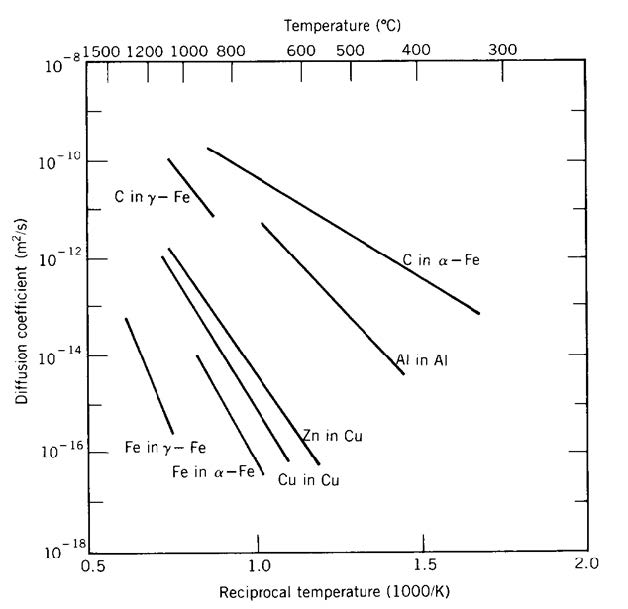
\includegraphics[scale=0.4,trim={0 0 0 0}]{figures/difTemp}

\begin{itemize}
	\item Influência da temperatura
	\item Influencia das especies em difusão
	\item Influencia das estruturas cristalinas 
\end{itemize}





\subsubsection{Difusão em materiais cerâmicos}


\begin{itemize}
	\item Mecanismos por lacunas
	\item Lacunas ocorrem em pares (defeito de Schttky)
	\item Difusão de íons de cargas opostas
	\item A condutividade elétrica de materiais cerâmicos é função do coeficiente de difusão.
\end{itemize}


